%        File: 24.03.20.tex
%     Created: пн мар 23 10:00  2020 M
% Last Change: пн мар 23 10:00  2020 M
%
\documentclass[algebra,twocolumn]{pum}
\listnumber{2}
\date{24.03.20}
\classname{8-Д}
\lesson{9:30-11:10 }
\begin{document}

\subsubsection*{Квадратичная функция}
Примером квадратичной функции служит функция $y=kx^2$. Ее графиком является некоторая кривая линия, которую называют параболой.

  \begin{center} 
    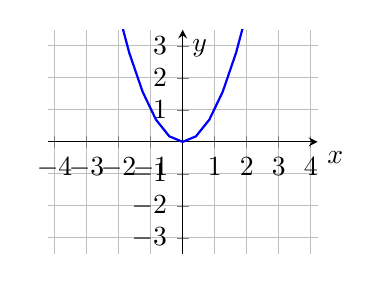
\begin{tikzpicture}
      \begin{axis}[
          scale=0.5,
          xmin=-1.5, xmax=1.5,
          ymin=-3.5, ymax=3.5,
          axis lines=middle,
          axis equal,
          grid=both,
          xtick distance=1,
          ytick distance=1,
          xlabel=$x$,
          ylabel=$y$,
          xlabel style={at={(ticklabel* cs:1)}, anchor=north west},
          ylabel style={at={(ticklabel* cs:1)}, anchor=north west}
        ]
        \addplot[blue,mark=none,thick=8pt] {x*x};
%  \addplot[blue,mark=none,thick=8pt, domain=-5:-0.2] {1/x};
%  \addplot[blue,mark=none,thick=8pt, domain=0.2:5] {1/x};
      \end{axis}
    \end{tikzpicture}
  \end{center}

Свойства графика квадратичной функции $y=x^2$:
\begin{enumerate}[nosep]
  \item График функции лежит в I и II координатных четвертях.
  \item График функции чертится сначала движением руки вниз, потом наверх с продвижение слева направо.
  \item У графика функции нет асимптот.
  \item Движение карандаша/ручки происходит без отрыва от бумаги.
\end{enumerate}

  \begin{exercises}
    \begin{question}
      Построить график функции
      \begin{multicols}{3}
        \begin{enumerate}[label=\arabic*)]
        \item $y=2x^2$ 
        \item $y=4x^2$ 
        \item $y=\frac{1}{2}x^2$ 
        \item $y=0.1x^2$ 
        \item $y=-2x^2$ 
        \item $y=-\frac{1}{2}x^2$ 
      \end{enumerate}
    \end{multicols}
  \end{question}
  \begin{question}
    Принадлежат ли графику каждой из построенных функций точки:\\
    A(1; 1), B(2; 16), C(-2; 4), D (10; 1).
  \end{question}
  \begin{question}
    По графику найти абсциссу точки графика построенных функций с ординатой: 10; -6; $\frac{10}{6}$. Сравнить это значение с числом, полученным из формулы.
  \end{question}
  \begin{question}
    По графику найти ординату точки графика построенных функций с абсциссой: -3; $\frac{1}{4}$; 0,2. Сравнить это значение с числом, полученным из формулы.
  \end{question}
\end{exercises}

\subsubsection*{Замечания по выполненным построениям}

\begin{center}
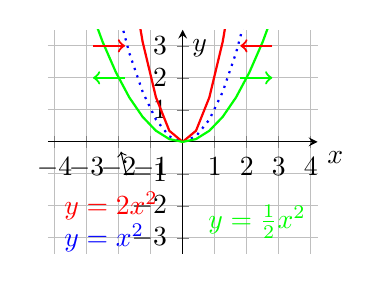
\begin{tikzpicture}
\begin{axis}[
    scale=0.5,
    xmin=-1.5, xmax=1.5,
    ymin=-3.5, ymax=3.5,
    axis lines=middle,
    axis equal,
    grid=both,
    xtick distance=1,
    ytick distance=1,
    xlabel=$x$,
    ylabel=$y$,
    xlabel style={at={(ticklabel* cs:1)}, anchor=north west},
    ylabel style={at={(ticklabel* cs:1)}, anchor=north west}
  ]
  \addplot[blue,mark=none,dotted,thick=8pt] {x*x};
  \addplot[red,mark=none,thick=8pt] {2*x*x};
  \addplot[green,mark=none,thick=8pt] {0.5*x*x};
  \node[blue,right] at (axis cs: -4,-3) {$y=x^2$};
  \node[red,right] at (axis cs: -4,-2) {$y=2x^2$};
  \node[green,right] at (axis cs: 0.5,-2.5) {$y=\frac{1}{2}x^2$};
  \draw[->,red,thick] (axis cs: 2.8,3) -- (axis cs: 1.8,3);
  \draw[<-,red,thick] (axis cs: -1.8,3) -- (axis cs: -2.8,3);
  \draw[<-,green,thick] (axis cs: 2.8,2) -- (axis cs: 1.8,2);
  \draw[->,green,thick] (axis cs: -1.8,2) -- (axis cs: -2.8,2);
  \node (horizont) at (axis cs: -2,0) {};
  \node (vertical) at (axis cs: 0,-2) {};
\end{axis}
\draw[->] (1,1) -- (horizont);
\end{tikzpicture}
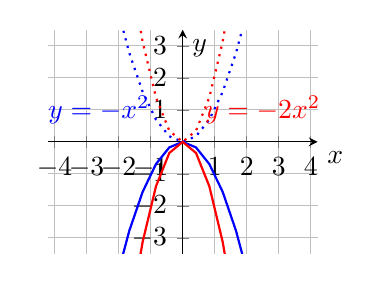
\begin{tikzpicture}
\begin{axis}[
    scale=0.5,
    xmin=-1.5, xmax=1.5,
    ymin=-3.5, ymax=3.5,
    axis lines=middle,
    axis equal,
    grid=both,
    xtick distance=1,
    ytick distance=1,
    xlabel=$x$,
    ylabel=$y$,
    xlabel style={at={(ticklabel* cs:1)}, anchor=north west},
    ylabel style={at={(ticklabel* cs:1)}, anchor=north west}
  ]
  \addplot[blue,mark=none,dotted,thick=8pt] {x*x};
  \addplot[blue,mark=none,thick=8pt] {-x*x};
  \addplot[red,mark=none,dotted,thick=8pt] {2*x*x};
  \addplot[red,mark=none,thick=8pt] {-2*x*x};
  \node[blue,right] at (axis cs: -4.5,1) {$y=-x^2$};
  \node[red,right] at (axis cs: 0.4,1) {$y=-2x^2$};
\end{axis}
\end{tikzpicture}
\end{center}

\begin{itemize}[nosep,leftmargin=0.5\labelwidth]
  \item Все построенные графики симметричны относительно оси ординат. Функции, графики которых обладают таким свойством называются \emph{четными}.
  \item Коэффициент пропорциональности $k$ сужает график функции по горизонтали, если он больше 1 и растягивает, если меньше 1.
  \item Если коэффициент пропорциональности отрицательный, то график функции является зеркальным отражением графика функции относительно оси абсцисс.
\end{itemize}


\pagebreak
\subsubsection*{Параллельный перенос}
Каждый из рассмотренных графиков проходит через точку $(0,0)$. Может так оказаться, что график какой-нибудь произвольной функции не проходит через эту точку, но при наложении его на прямую, параболу или гиперболу в точности повторяет начертание одной из них. Аналитически это означает, что можно выполнить замену переменной таким образом, что в новых обозначениях мы получим функцию график, которой проходит через точку $(0,0)$. Геометрически это означает параллельный перенос всех точек графика функции на какое-то расстояние. А замена вводится так:
\begin{equation*}
  u=x-a,\quad v=y-b
\end{equation*}
При такой замене вершина параболы и точка пересечения асимптот гиперболы переходит в точку $(a,b)$.

  \begin{exercises}
    \begin{question}
      \label{qu:graph1}
      Построить графики функций, где перенос задан явными выражениями:
      \begin{multicols}{2}
        \begin{enumerate}[label=\arabic*)]
        \item $y=x-2$ 
        \item $y+2=x$ 
        \item $y=\frac{1}{x+3}$ 
        \item $y-1=\frac{1}{x}$ 
        \item $y=(x-2)^2$ 
        \item $y+5=-x^2$ 
      \end{enumerate}
    \end{multicols}
  \end{question}
    \begin{question}
      \label{qu:graph2}
      Построить графики функций:
      \begin{multicols}{2}
        \begin{enumerate}[label=\arabic*)]
        \item $y=\frac{2x-2}{3}$ 
        \item $y=5\frac{x-2}{3}$ 
        \item $y=\frac{3}{-2x+3}$ 
        \item $y=\frac{x+1}{x-1}$ 
        \item $y=x^2+4x+4$ 
        \item $y=x^2+2x+2$ 
      \end{enumerate}
    \end{multicols}
  \end{question}
  \begin{question}
    Принадлежат ли графику каждой из построенных функций точки:\\
    A(2; 1), B(12; -4), C(0,3; -16), D (0,4; -120).
  \end{question}
  \begin{question}
    По графику найти абсциссу точки графика построенных функций с ординатой: 10; -6; $\frac{10}{6}$.
  \end{question}
  \begin{question}
    По графику найти ординату точки графика построенных функций с абсциссой: -3; $\frac{1}{4}$; 0,2.
  \end{question}
  \begin{question}
    Найти точки пересечения с осями координат графиков функций, построенных в упражнении \ref{qu:graph1} 
  \end{question}
  \begin{question}
    Найти точки пересечения с осями координат графиков функций, построенных в упражнении \ref{qu:graph2} 
  \end{question}
  \begin{question}
    Отразить график функций из упражнения \ref{qu:graph1}, \ref{qu:graph2} относительно оси ординат.
  \end{question}
  \begin{question}
    Отразить график функций из упражнения \ref{qu:graph1}, \ref{qu:graph2} относительно оси абсцисс.
  \end{question}
  \begin{question}
    Отразить график функций из упражнения \ref{qu:graph1}, \ref{qu:graph2} относительно начала координат.
  \end{question}
\end{exercises}

\bigskip
\subsubsection*{И еще одно определение}
Функция, график которой симметричен относительно начала координат, называется \emph{нечетной}. Примером таких функций являются прямая, проходящая через начало координат, и гипербола асимптоты, которой пересекаются в начале координат.

\end{document}


